\chapter{Desenvolvimento do trabalho}

Este capítulo tem como objetivo explicitar quais foram as decisões de projeto que foram tomadas ao longo do desenvolvimento do sistema.

\section{Tecnologias utilizadas}


\subsection{ATmega328P}

A placa de Arduino foi escolhida para este projeto, pelos motivos citados a seguir:

\begin{itemize}
    \item É fácil de ser usada, o que ajuda na ideia de \textit{open-hardware}.
    
    \item Memória programável já dentro do sistema (algumas pacas AT não têm).
    
    \item Não é caro (maior parte do custo será nos componentes mecânicos).
    
    \item Consumo de energia baixo (22mW) em relação à potência proposta (de 1W).
\end{itemize}
\subsubsection{Analise de Capacidade}

Foi necessário calcular ser o microcontrolador seria capaz de realizar o processamento esperado. Iniciamos sabendo que no pior caso serão necessários 60 atualizações por segundo, ou seja o sistema deve responder em \SI{1666.6}{\micro\second}, seja \SI{555.5}{\micro\second} cada cada um dos 3 eixos.

A leitura da porta analógica leva \SI{100}{\micro\second} \cite{Datasheet}, e a resposta do motor de passo será do mesmo valor, considerando um motor de 10000 passos por segundo. Sendo assim,  cada eixo tem \SI{355.5}{\micro\second} de tempo para calculos, num micro controlador com \textit{clock} de \SI{20}{\mega\hertz}

Dessa forma, a placa deve ser capaz de realizar 5100 ciclos, com um CPI de 2 para a maior parte das operações e um pipeline de 2 instruções \cite{Datasheet} podemos estimar um ISP de 1, ou seja é possível realizar 5100 instruções a cada ciclo, o que é o suficiente para as operações necessárias, já que são em sua maioria somas e substrações.  

Podemos ver as operações mencionadas acima na figura \ref{fig:cal_tempo}.

\begin{figure}[H]
    \centering
    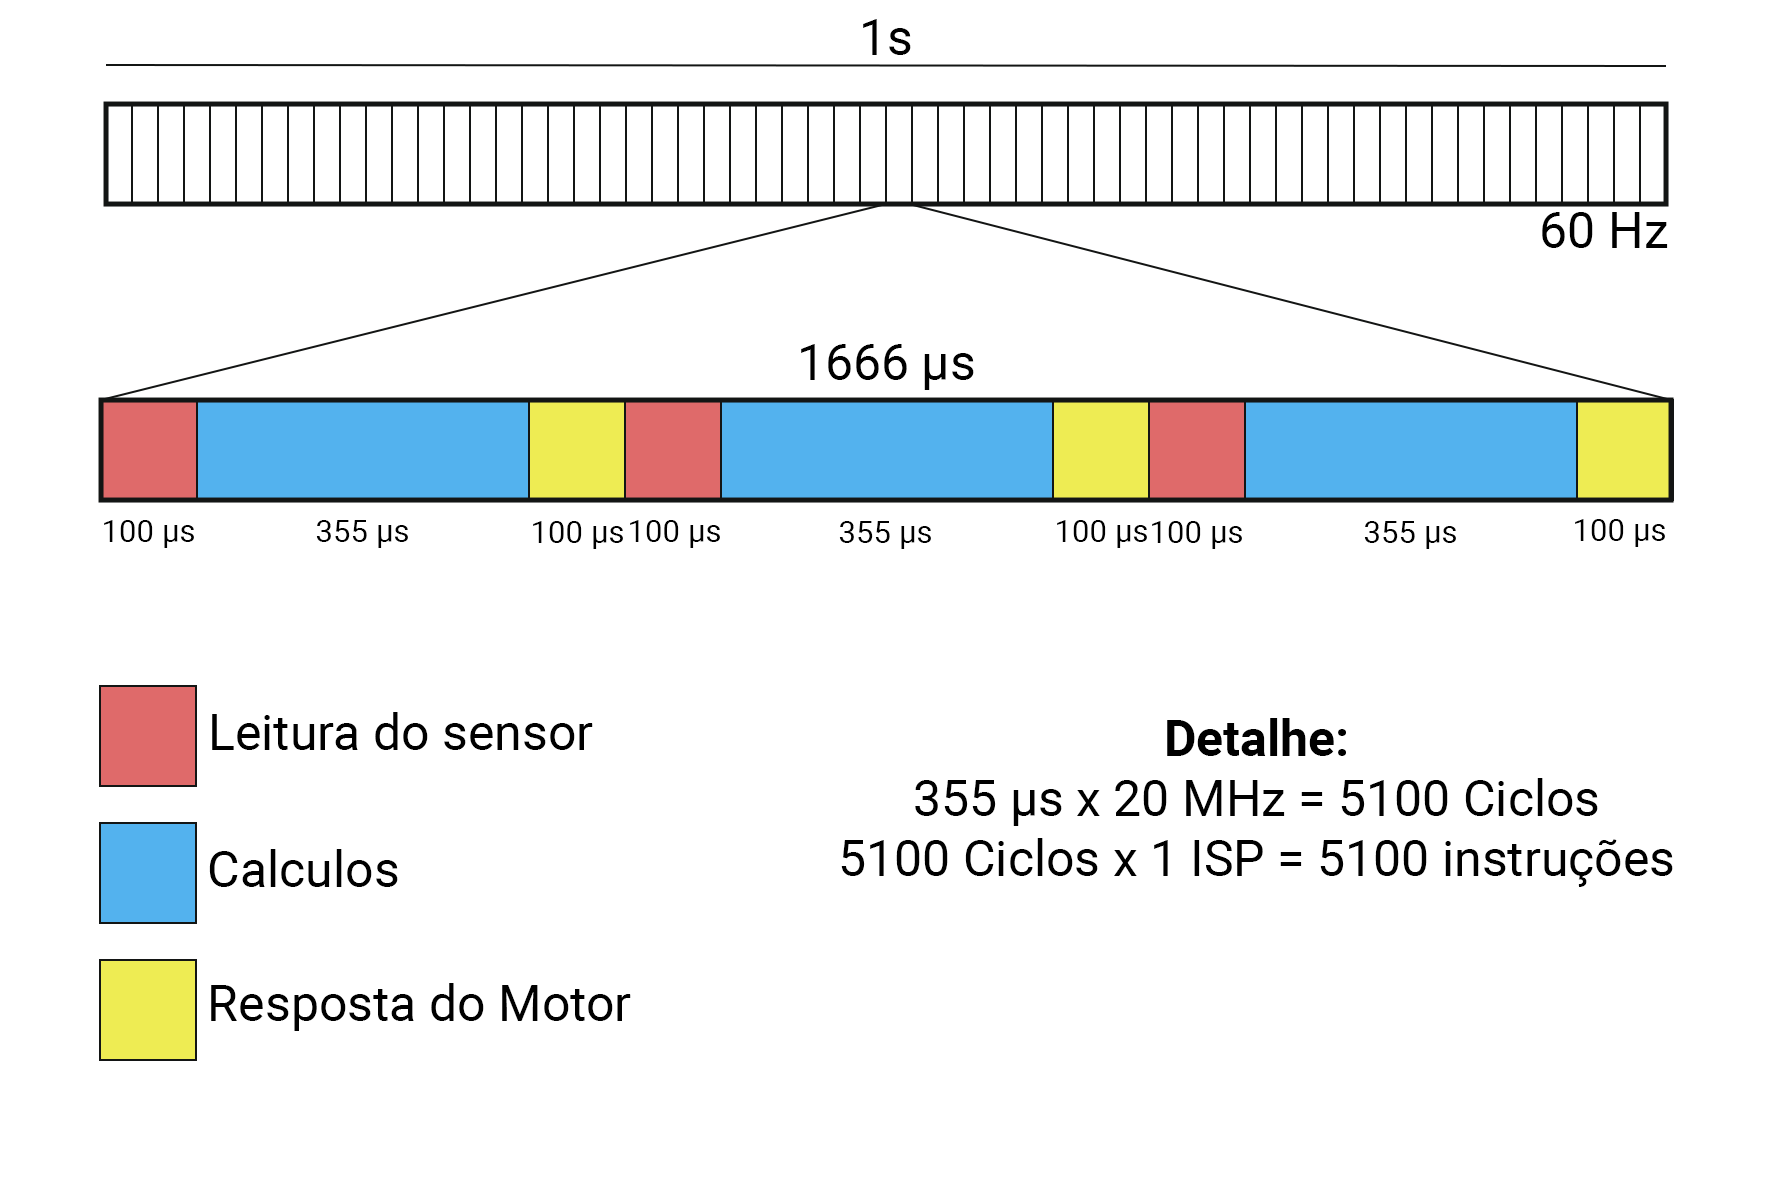
\includegraphics[width=1\textwidth,angle=0]{figures/calculos de tempo.png}
    \caption{Visualização dos tempos para cada etapa de processamento}
    \label{fig:cal_tempo}
\end{figure}


% \subsubsection{Análise}


\subsection{Sistema Operacional}
Como o projeto requer controle em tempo real da câmera, é necessário usar-se um RTOS (real time operating system).
Entre os SOs observados pelo grupo, o mais adequado para o controlador Gimbal é o ARM OS, pois é o recomendado pela ATMEL para RTOS em suas placas.

Nota-se que o ARM OS RTOS exige copilação usando o mbed, no entanto isso não deve ser problema, já que esse é disponível gratuitamente online. 

\subsection{Interface}
SPI (GPIO das placas feitas pela Arduino):
Giroscópio: dados posicionais
Acelerômetro: dados posicionais
Botões (ao menos dois): interface com o usuário
LED (depuração): interface com o usuário
USB:
Carregamento: fazer o código rodar no Arduino 
Depuração: do código na placa

\subsection{Ambiente de desenvolvimento e depuração}
Usaremos as bibliotecas de cada sensor e motor a ser usado, para facilitar a integração
Não há necessidade de sistema de arquivos, já que os dados são tratados ativamente
Usaremos os drivers de interface com o GPIO fornecidos pelo SO
A depuração será feita em cada camada de maneiras diferentes: 
Simulação → aplicação 
QEMU → SO 
LEDs → hardware 

\section{Projeto e implementação}

\subsection{Design}

\begin{figure}[H]
    \centering
    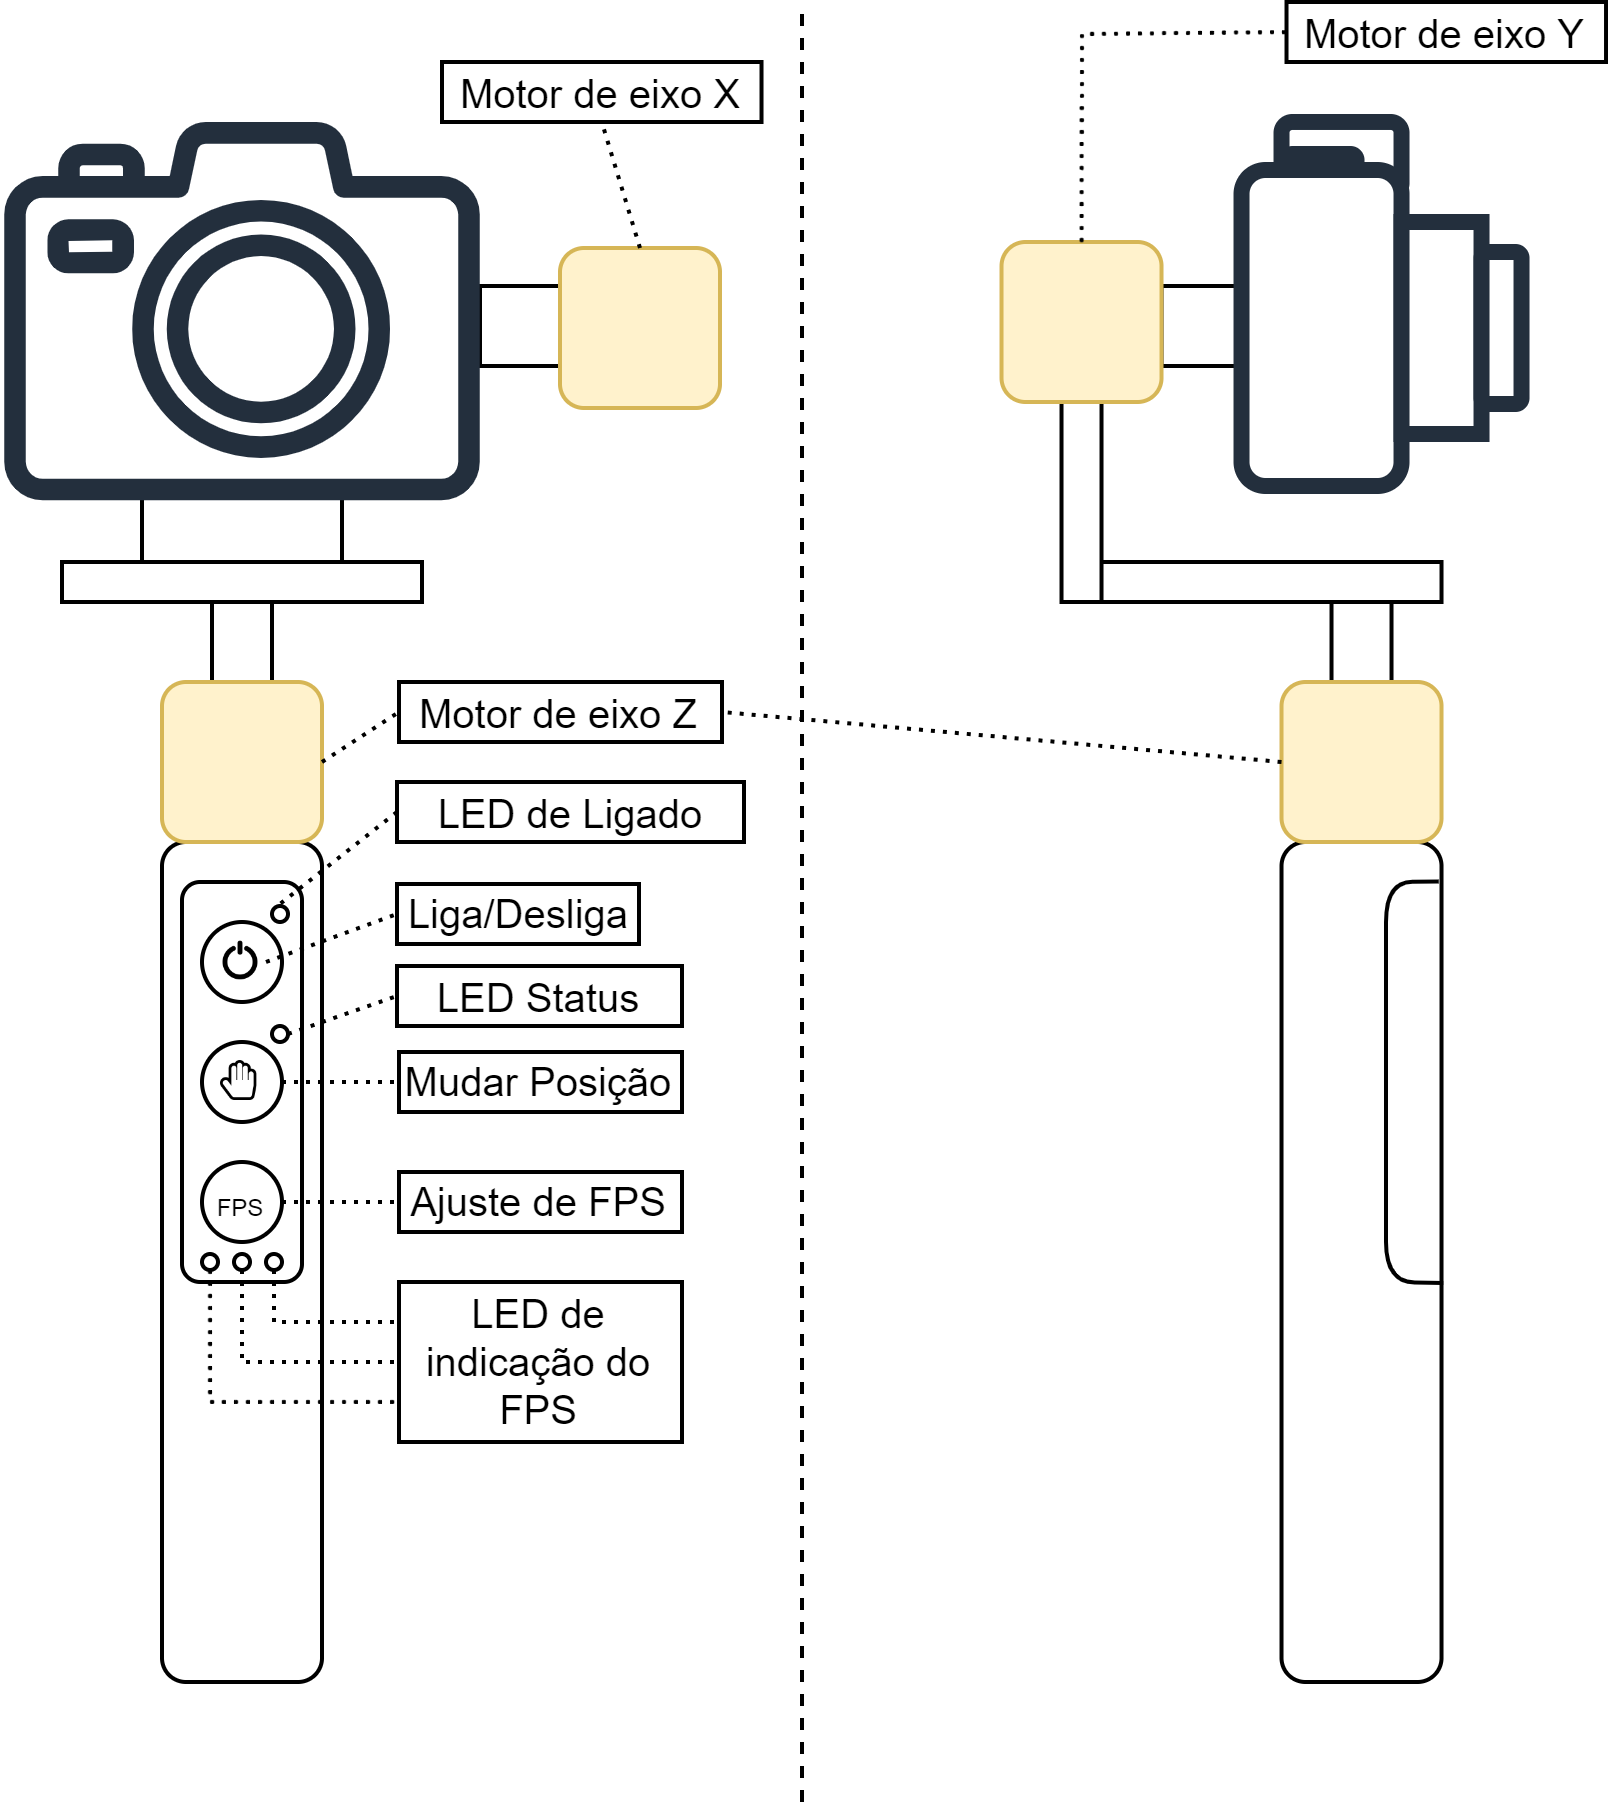
\includegraphics[width=1\textwidth,angle=0]{figures/Design-Page-1.png}
    \caption{Design básico do projeto}
    \label{fig:design_basico}
\end{figure}

\begin{figure}[H]
    \centering
    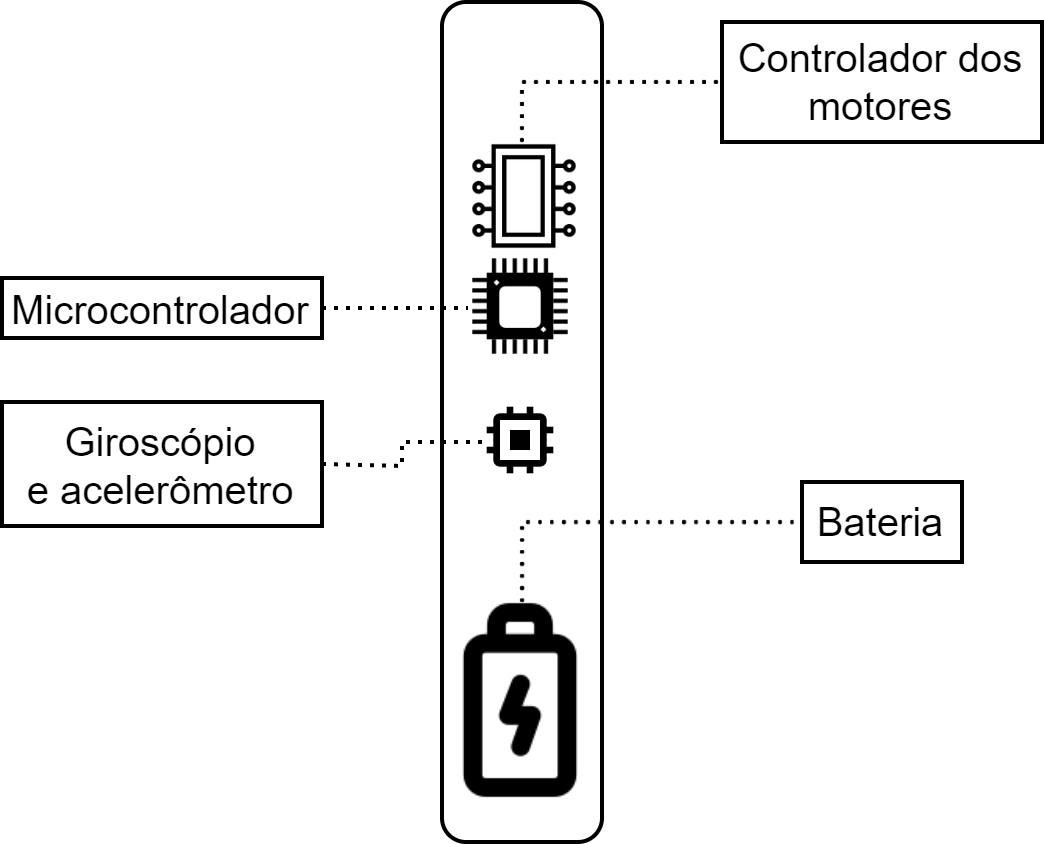
\includegraphics[width=1\textwidth,angle=0]{figures/Design-Page-2.png}
    \caption{Design básico do interior do projeto}
\end{figure}

\section{Testes e avaliação}

Um plano de testes inicial foi elaborado para que o sistema possa ser validado quando estiver pronto.

\begin{itemize}
    \item Teste do Sensor: verifica-se o código somente com um sensor e vendo o resultado de posição na tela.
    
    \item Teste de 1 eixo: Faz-se o teste com somente um eixo, essencialmente um pendulo invertido.
    
    \item Teste de 3 eixo: Faz-se o teste com todos os eixos, mas sem o acabamento.
    
    \item Teste de final: Produto pronto será testado.
\end{itemize}


